\documentclass[preprint,12pt,nopreprintline]{elsarticle}
\usepackage[T1]{fontenc}
\usepackage{lmodern,microtype,graphicx,booktabs,amsmath,amssymb,array,tabularx,xurl}
\usepackage[hypertexnames=false]{hyperref}
\hypersetup{pdfauthor={Author review draft},pdftitle={Execution State and Cost Boundaries of Reference-Preserving Speculative Decoding},pdfsubject={JSA structural revision v0.13.0, not submitted}}
\setlength{\emergencystretch}{2em}
\newcommand{\R}{R}\newcommand{\M}{M}\newcommand{\C}{C}
\makeatletter
\def\ps@pprintTitle{\let\@oddhead\@empty\let\@evenhead\@empty\def\@oddfoot{\hfil\thepage\hfil}\let\@evenfoot\@oddfoot}
\makeatother
\begin{document}
\begin{frontmatter}
\title{Execution State and Cost Boundaries of Reference-Preserving Speculative Decoding}
\date{}
\author{Author-review draft}
\begin{abstract}
Speculative decoding changes both the numerical trajectory and the cost of language-model execution. We study their interaction in quantized consumer-system deployments. Early interventions and a matched target-only bridge show that exact output prediction does not establish useful repair or a need for complex reproduction machinery. Natural retained-state crosses on CUDA and Vulkan then distinguish current-path effects, state effects, and local interactions despite equal committed prefixes. A finite RTX target-attention constraint preserves full reference responses on 24 project-unused inputs. Generation speed is 1.170 times ordinary decoding and 1.169 times matched draft-free execution. Resident-request speed is 1.742 times ordinary but only 1.035 times matched execution: the target-path change already provides 1.683 times without speculation. Wider fixed-capacity drafting and B570 endpoint repair qualify while losing performance. Historical M4 and 358H studies expose limits on adaptation and draft-only optimization. The contribution connects execution diagnosis, finite repair design, and paid two-baseline evaluation through positive cases and qualified counterexamples. The numerical recipes and mechanism evidence remain deployment-specific.
\end{abstract}
\begin{keyword}
speculative decoding \sep execution state \sep numerical consistency \sep runtime architecture \sep performance evaluation \sep consumer systems
\end{keyword}
\end{frontmatter}
\section{Introduction}
Speculative decoding changes how a language-model runtime executes work, not only how many target calls it makes. A draft proposes tokens, the target verifies several positions, and the runtime commits or rolls back state before continuing. The transformation provides useful acceleration only when the resulting execution satisfies its output requirement and the saved target work exceeds the added work~\cite{leviathan2023}. On quantized consumer systems, these conditions can fail separately.

For applications that must reproduce a selected greedy reference, equal committed token prefixes are an incomplete description of execution. Prefill and verification can use different numerical shapes, and previous calls can leave different numerical cache contents. A deviation at the next decision may depend on retained state, the current recipe, or their interaction. A repair chosen without separating these factors may reproduce one case and introduce another deviation. Even a repair that qualifies complete outputs can remove the performance advantage it was intended to preserve.

The same difficulty appears in the cost baseline. A repair can change target prefill or continuation before speculation is enabled. Comparing repaired speculation only with the original decoder can attribute this target-path improvement to speculation. Comparing only with a matched target-only path answers a different question and can hide the full deployment change. Both paid comparators are needed to interpret the result.

This paper examines these design decisions through controlled consumer-system studies. Early B570 and RTX interventions test whether output prediction establishes a useful repair. A matched RTX bridge tests whether a simpler draft-free execution explains the intervention output. Later natural-state crosses distinguish the state carried into a decision from the recipe used at that decision. A finite RTX attention-layout family then supplies a qualified repair, evaluated against ordinary and matched draft-free execution. Width tests, B570 costs, and historical M4 and 358H campaigns examine where qualification fails to produce a useful operating point.

The studies have different evidence roles. Selected-boundary interventions identify local effects; exposed panels guide repair selection; an input expansion checks a frozen recipe on project-unused inputs; paid sessions evaluate qualified outputs. We retain these distinctions rather than pooling all requests into a success rate. The four platforms are separate system cases, not four matched replications of one mechanism.

Our contribution connects execution-state consistency, repair scope, and paid system cost:
\begin{enumerate}
\item \textbf{Diagnostic evidence for separating state and current execution.} Natural donor-state crosses on CUDA and Vulkan reveal path effects, state effects, interactions, and selected-boundary nulls. Earlier prediction and simple-baseline results show why output reproduction alone cannot select a useful repair.
\item \textbf{A bounded repair-design case.} A query-layout constraint on target prefill and continuation is inclusion-minimal within a tested four-switch family on RTX. The frozen recipe qualifies complete reference responses on 24 project-unused MBPP inputs. This is a local graph transformation, not a portable determinism theorem.
\item \textbf{Qualified cost evidence and counterexamples.} RTX generation improves against both ordinary and matched draft-free execution. Much of its ordinary-reference request gain is already available without speculation. Wider fixed-capacity drafting and a B570 endpoint repair qualify while losing performance; M4 and 358H show limits on adaptation and draft-only optimization.
\end{enumerate}

The system-design lesson concerns three connected decisions: which execution state and path require control, which finite constraint preserves the registered output, and which baseline reveals operational value. Existing work establishes state consistency, numerical shape sensitivity, and verification overhead. We do not claim their discovery, a new general algorithm, or a universally optimal constraint. The additional evidence links these concerns within measured deployments and includes repairs that do not pay.

The paper defines the runtime and prior-work context, then the execution and measurement contracts. Its results follow diagnosis, repair design, and cost evaluation; the discussion extracts reusable design decisions while preserving deployment-specific limits.


\section{Runtime Architecture and Related Work}
\label{sec:background}
\subsection{The speculative execution transaction}
A speculative iteration has four relevant stages. The draft first extends the committed prefix with candidate tokens. The target evaluates candidate positions, often in a multi-token call. Acceptance, correction, and bonus sampling determine the next committed tokens. The runtime then reconciles cache positions and pending computation before the next iteration. Its target cache must represent the committed trajectory after rejected candidates are removed or repaired.

The ordinary greedy reference advances through its own sequence of prefill and continuation calls. Identical token IDs so far do not certify identical numerical histories. Allocated microbatch capacity, occupied positions, attention query layout, and output reservation can affect the current computation. These quantities must not be conflated: changing capacity does not prove every call occupies that capacity, and changing a whole recipe does not isolate a single operator.

We study quantized Qwen3 deployments with native proposals and recorded backends. The late RTX graph constrains non-flash attention layout while keeping other target operations batched. B570 uses a separately qualified Vulkan phase-binding recipe. Historical M4 and 358H retain their own interfaces. This is a software execution study on consumer hardware, not a hardware-only comparison.

\subsection{Numerical preservation and state intervention}
Batch-invariant inference constrains numerical reductions~\cite{thinkingmachines}. LLM-42 combines fixed-shape verification, consistent KV state, and selective deterministic requests~\cite{llm42}. Stage-Replay holds prefixes fixed and performs bidirectional cache transplantation~\cite{stagereplay}. Vosti specifies and verifies system-level determinism~\cite{vosti}, a stronger guarantee than finite token or endpoint qualification. MarginGate studies calibrated sparse verification~\cite{margingate}.

State intervention has precedent. Our additional measured factor is the current native recipe crossed with naturally retained state, followed by finite repair qualification and paid ordinary/matched comparisons. We have no shared-contract implementation comparison with those methods. The crosses cannot establish superiority to a verified deterministic runtime; sampled-token agreement does not establish equal logits or caches.

\subsection{Performance and heterogeneous drafting}
Speculative sampling~\cite{leviathan2023}, heterogeneous drafting~\cite{dovetail,duodecoding}, and adaptive depth~\cite{turbospec,banditspec} are established directions. Consumer numerical deviations and serialization costs are documented~\cite{lossless}. \emph{Performance or Illusion?} examines verification costs and performance limits in a production engine~\cite{illusion}. Our experiments connect reference-qualified repair scope with the distinction between changing a target path and adding speculation on that path.

Contextual uncertainty-based verification allocation is studied by HeteroSpec~\cite{aclheterospec}. Our question concerns the execution state, repair scope, and cost of reproducing a registered reference.


\section{Execution and Measurement Contracts}
\label{sec:contracts}
\subsection{Output as a registered system requirement}
Fix model weights, tokenizer, prompt format, sampler, runtime, backend, and output endpoint. Let $R(x)$ be the paid ordinary reference for input $x$. Qualification compares token IDs, committed length, terminal token when available, and stop reason. It measures reference reproduction, not program correctness, equal logits, or distributional equivalence.

The RTX input expansion checks the full saved response array through runtime end-of-generation (EOG) or the token cap. B570 registers the prefix through the first runtime EOG or token 128. Its raw response can contain a suffix while satisfying that endpoint; actual suffix work remains in candidate cost. Endpoint preservation and raw-array equality are separate results.

This contract fixes what a repair must preserve before costs are interpreted. A faster execution with shorter or divergent output is not a qualified speedup. Finite qualification supports the recorded inputs and configuration, not arbitrary future inputs.

\subsection{The state--current-path cross}
At a naturally reached boundary, let $p$ be the committed token prefix, $s$ the retained numerical/runtime state, and $e$ the current recipe. The decision is
\begin{equation}
d=F(p,s,e).
\end{equation}
Holding $p$ fixed and crossing two natural donors $s_0,s_1$ with two current recipes $e_0,e_1$ yields four observations. Within-row differences identify a current-recipe effect for that donor. Within-column differences identify a donor-state effect for that recipe. A recipe effect under only one donor is a local interaction. A discrete null does not imply equal continuous scores.

A valid cross requires cache ownership and position alignment, faithful restoration, and a shared continuation boundary. Own-path shams check whether restoring each donor under its own recipe reproduces the native decision. Natural donors use live proposals rather than a future proposal tape supplied to the candidate. These controls support local interventions; they do not isolate a unique operator or prove complete counterfactual suffix equality.

\subsection{Repair placement and the matched comparator}
A repair constrains specific execution phases rather than merely declaring execution serialized or changing a global capacity option. The RTX family has four switches: target prefill, target continuation, draft prefill, and draft continuation. A passing switch set determines which phases require the local attention-layout constraint on the measured panel.

The system boundary extends beyond verification. Restored output requires valid acceptance, committed state, stopping, and subsequent continuation. Leaving the draft unconstrained in a passing panel does not license arbitrary draft behavior in every implementation. B570 changes several runtime settings together and is evaluated as a whole recipe.

Three paths assess the repair:
\begin{itemize}
\item $R$: the paid ordinary reference without a draft;
\item $M$: the candidate's target path and prefill configuration, without a draft;
\item $C$: that target path with native drafting and verification.
\end{itemize}
$R/C$ measures the full deployment change; $M/C$ measures speculation's increment on the repaired path. $R/M$ exposes the target-path change available without speculation. A qualified $R$ is not necessarily the fastest possible ordinary decoder.

\subsection{Cost estimators and their interpretation}
For task $i$, take the median absolute time $t_{i,b}$ or $t_{i,c}$ within each condition, then the ratio. The late RTX estimator is
\begin{equation}
S_{b/c}=\exp\left(\frac{1}{n}\sum_{i=1}^{n}\log\frac{t_{i,b}}{t_{i,c}}\right).
\label{eq:gm}
\end{equation}
Values above one favor the candidate. Repetitions are collapsed before the ratio, not counted as independent inputs. Descriptive bootstrap intervals resample tasks after this collapse. For common tasks, timers, and aggregation,
\begin{equation}
S_{R/C}=S_{R/M}S_{M/C}.
\label{eq:identity}
\end{equation}
This identity links comparisons, not additive component costs. Request minus generation time or differences between ratios cannot identify attention, transfer, synchronization, or host overhead without independent profiling.

Late RTX generation excludes prompt processing, its first-sample boundary, and some final bookkeeping. Resident-request time covers complete HTTP response receipt and parsing, excluding loading, warmup, and shutdown; asynchronous post-response cleanup is not certified inside it. Historical studies retain their boundaries and, on 358H, a different median-of-paired-ratios estimator.

Qualification precedes the speed claim. Both aggregates and task variation matter: a positive geometric mean can coexist with regressions. These measurements characterize operating points, not global optimality or production concurrency.


\section{Study Design and Evidence Organization}
\label{sec:studies}
\subsection{Systems and research questions}
Late RTX studies use an RTX 5070 Ti Laptop, Qwen3-8B/Qwen3-0.6B Q8\_0, the frozen non-flash CUDA graph, greedy sampling with seed 123, context 4096, 24 host threads, and one slot. B570 uses Qwen3 with its Vulkan recipe. Historical M4 uses Metal; 358H combines a Vulkan target with CPU or NPU drafting, including symmetric INT4 OpenVINO drafting. Hardware, runtime, backend, and interfaces jointly vary.

We ask three questions:
\begin{enumerate}
\item Which decision changes follow retained state, the current recipe, or their interaction, and what does a simpler execution already explain?
\item Which phases need a finite constraint to qualify the reference, and where does that repair cease to qualify?
\item When qualification holds, does paid cost improve against ordinary and matched draft-free execution, and what simpler alternative captures the available benefit?
\end{enumerate}
These questions organize the cases; experiments are not pooled into a matched platform comparison.

\begin{table}[t]
\centering\small
\caption{Evidence roles. Counts remain campaign-specific; the supplement gives the expanded inventory.}
\label{tab:studies}
\begin{tabularx}{\linewidth}{@{}p{.20\linewidth}XX@{}}\toprule
Role & Main evidence & What it establishes\\\midrule
Prediction and simpler paths & B57024, RTX43, fresh RTX19 bridge, offline selection & Reproduction, repair/regression, and need for added complexity\\
Local diagnosis & RTX donors and width boundary; B570 crosses & Selected-state/current-recipe effects with shams\\
Finite repair & RTX 16 masks and exposed scope costs & Qualification and inclusion-minimal scope in a fixed family\\
Input expansion & RTX24, four conditions, four repetitions & Frozen-recipe qualification and paid two-baseline costs\\
Cost boundaries & Width, B57015, historical M4/358H & Qualified failures and bounded opportunities\\\bottomrule
\end{tabularx}
\end{table}

\subsection{Exposure, qualification, and timing}
RTX separates four exposed HumanEval probes~\cite{humaneval}, the 16-mask factorial, exposed qualification/cost panels, a frozen MBPP expansion~\cite{mbpp}, and width/length tests. Exposure accounting before reference generation identifies 24 eligible MBPP inputs. Project-unused means unused in accessible experiment history, not absent from pretraining or a new model family. They become exposed for later analysis once measured.

The expansion has 24 tasks, four conditions, and four repetitions: 384 formal paid requests and 16 excluded warmups. All conditions have 96 qualified responses, with stable references. Output lengths range from 11 to 128; 23 tasks end at EOG and one at the cap. Capture is off. Four condition-specific resident processes per round use rotated condition and task orders; recorded cache reuse is zero. A separate request-reset study adds no independent expansion inputs.

Auxiliary diagnostic forwards are not latency measurements. Discovery and screening costs are not pooled with confirmation. B570's endpoint rule does not certify RTX full arrays; historical parsed-text checks do not acquire the strength of later direct-ID checks retrospectively.

\subsection{Reconstruction and access}
This reconstruction organizes saved experiments and launches no inference, GPU campaign, or warmup. The late 26-file bundle is preserved byte-for-byte. Historical source extracts are matched to latest repository blobs. The build recomputes public RTX costs, qualification-hash joins, B570 costs, and selected workload summaries.

Arithmetic validation inherits original-host verification of private outputs and timers. It does not independently reopen every raw archive, weight, or runtime. The source package provides calculations and provenance boundaries; full independent hardware replay is a different task.


\section{Diagnostic Evidence: Prediction, Simple Paths, and Natural State}
\label{sec:early}
\subsection{Prediction closure does not select a useful intervention}
The early studies distinguish prediction/native agreement from reference agreement. B570 changes target prefill UB1-to-UB128 with the prescribed first-pending sample and state handoff; continuation and draft remain UB1. On an exposed 24-task cohort, baseline and intervention predictions each match all 72 repeated native arrays. Reference agreement rises from 60/72 to 72/72: four known deviations recover without a new deviation among 20 controls.

This does not isolate KV alone. Transferred state includes pending logits, positions, and a post-accept sampler clone. The result concerns the recorded intervention, not arbitrary prefill-only repair or performance benefit.

RTX changes target continuation UB2-to-UB1 while retaining recorded prefill, draft, and caller grouping. Predictions reproduce both native conditions on 19 exposed HumanEval tasks and 24 statically selected MBPP tasks: 57 and 72 repeated arrays per condition. Yet HumanEval/15 repairs, /25 regresses, and /18 stays divergent. HumanEval reference agreement remains 51/57, or 17/19 tasks. MBPP remains 66/72, with two persistent failures. An unchanged aggregate hides opposing effects.

One persistent failure also changes its complete output. MBPP/304 retains 47 IDs but changes 488 to 481 at zero-based position 33 while staying divergent. Reference failure, output change, and no-op are distinct. These results motivate controlling execution state and phase; they do not validate the predictor as a repair selector.

\subsection{The ordinary target-only bridge}
A fresh comparison tests whether ordinary draft-free $U_2$ reproduces the RTX intervention $N_1$. It uses the same 19 exposed HumanEval tasks, three conditions, and three fresh-process repetitions: 171 formal runs. Relevant numerical threads are matched at 24; condition order rotates, and no process or KV state is reused. $U_2$ uses its own prefill and continuation, without draft, transplant, proposal tape, or reference answer.

$U_2=N_1$ on all 57 complete arrays and strict stop boundaries. $U_2=N_0$ and $N_0=N_1$ each hold for 51/57 arrays. The changed tasks are the repair and regression above; the other 17 are output no-ops. Each condition is repeat-stable on all 19 tasks, while all retain 17/19 reference agreement.

The simpler path reproduces both nontrivial changes on this cohort. Allocated UB2 does not require two occupied continuation tokens: $U_2$'s observed continuation batches contain one token. Live $U_2$ graph tensors and KV/logits are unavailable, so output equality is not a state-equivalence theorem. The complex predictor is unnecessary for this particular reproduction objective; no timing or general predictive advantage follows.

\subsection{A bounded negative selection result}
An existing-record analysis tests whether paid proxy screening adds a supported configuration-selection capability. A proposed state-fingerprint rule lacks aligned state and a repair direction for implementation. A charged proxy-and-verification replay compares available outcomes with direct enumeration, without exposing unqueried labels.

On RTX19, enumeration and proxy screening both abstain and use 114 post-common-acquisition record equivalents. On B57024, direct verification selects the sole candidate with 72 records; proxy screening selects it with 144. These are retrospective acquisition equivalents, not latency or new inference. MBPP target-only counterfactuals are unavailable and remain unknown.

For a sole accepted action, screening adds proxy/setup work unless it supplies an otherwise unavailable capability or rejection saving. No matched timing establishes that benefit here. Diagnostic fidelity, repair utility, and operational value therefore need separate evidence before retaining additional machinery.


\subsection{Natural state and current execution}

\label{sec:cross}
\subsubsection{RTX: path effects and local interactions}
Four previously exposed HumanEval probes use naturally reached donor states at equal committed prefixes. Across repetitions, 24 donors generate 48 state/current-path forks with 24 own-path shams. Auxiliary probe forwards are separately charged and are not speed measurements. Restoring and continuing an own-path state checks that the manipulation itself reproduces the native decision.

At HumanEval/15, the final verification/bonus decision changes with the current UB2 versus UB1 call under both donors. At HumanEval/25, only the combination of the N1 donor and current UB1 call changes the sampled decision. The latter is an interaction, not a state-only explanation. At the chosen boundaries of /18 and /31, neither intervention changes the discrete decision. A null at these boundaries does not prove trajectory-wide invariance.

\begin{figure}[t]
\centering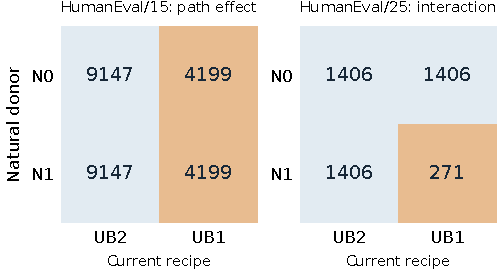
\includegraphics[width=0.62\linewidth]{figures/state_path_cross.pdf}
\caption{RTX natural-state crosses at fixed committed prefixes. /15 shows a current-path effect under both donors; /25 changes only for N1 with UB1. Cells display the discriminating sampled token ID: the third decision for /15 and the first for /25. Colors group equal IDs within each task. These selected cells are local causal observations.}
\label{fig:statepath}
\end{figure}

The donors' prompt K/V tensors agree in all 12 compared pairs, while 70 of 72 generated-prefix tensor comparisons differ. First-layer logical K/V remain equal in the tested pairs.  

The expanded width study supplies another case. MBPP/229 at a natural 47-token prefix fails at wide UB6 verification. Real donor-state crosses under two current query layouts flip EOG argmax with the state; current layout changes continuous scores without independently flipping argmax in the measured cells. Four shams reproduce their own decisions. Two cap contexts are two observations of one task, not two independent counterexamples. This case connects a numerical-state boundary to a wider qualified-execution search without claiming a uniquely causal CUDA kernel.

\subsubsection{B570: a different recipe and the same questions}
On B570, six natural-state crosses with 12 own-path shams cover three tasks in repeated contexts. Byte-validated round trips and KV ownership checks support genuine donor-state manipulation. HumanEval/145 and /42 show local state--whole-recipe interactions. MBPP/72 shows a donor-state effect while its two current-recipe columns are identical controls. It cannot count as an independently varied current-path effect.

Table~\ref{tab:cross} shows representative raw argmax IDs, whose numeric magnitudes have no metric interpretation. The current B570 recipes change microbatch and output-reservation behavior together. The matrix therefore does not isolate one operator. Subsequent counterfactual complete continuations are not available for these cross cells; endpoint recovery is demonstrated separately by native full requests.

\begin{table}[t]
\centering\footnotesize\setlength{\tabcolsep}{3pt}
\caption{Representative B570 $2\times2$ argmax matrices. Rows are natural donor states; columns are the recorded current recipes. /72 has duplicate columns. Cases are local evidence, not prevalence estimates.}
\label{tab:cross}
\begin{tabular}{lcc}\toprule
Task & Donor 0: $(e_0,e_1)$ & Donor 1: $(e_0,e_1)$\\\midrule
HumanEval/145 & $(71465,279)$ & $(279,279)$\\
HumanEval/42 & $(432,1817)$ & $(1817,1817)$\\
MBPP/72 & $(320,320)$ & $(308,308)$\\\bottomrule
\end{tabular}
\end{table}

Together the two GPUs support the portability of the \emph{experimental question}: equal prefixes do not remove the need to control retained state and the current recipe. They do not demonstrate that one constraint, matrix pattern, or parameter choice transfers unchanged between CUDA and Vulkan.


\section{Finite Repair Design on RTX}
\label{sec:repair}
\subsection{Local attention layout and phase scope}

The RTX implementation changes the query layout of the Qwen3 non-flash attention subgraph using existing ggml views and CUDA operations. Query columns are represented in the batch dimension so that attention follows the selected scalar-query structure; projection and feed-forward operations retain their batched execution. This is a local graph transformation, not a new CUDA kernel or architecture-independent arithmetic proof.

Four switches apply the constraint to target prefill, target continuation, draft prefill and draft continuation, encoded by bits 1, 2, 4 and 8. The exposed factorial contains 16 masks, four probes and two repetitions, totaling 128 complete requests. Masks 3, 7, 11 and 15 pass every registered reference endpoint. Mask 3 is inclusion-minimal within this finite family. /15 and /31 pass all masks; /25 needs either target phase; /18 needs both. Draft constraints are unnecessary for qualification on this panel. 

Mask 3 is chosen by output qualification, not observed speed. On 19 exposed tasks, the subsequent six-repetition panel yields 1.27808$\times$ generation and 1.11298$\times$ resident-request speed against matched target-only execution. Removing draft constraints relative to mask 15 adds only 1.00357$\times$ generation and 1.02569$\times$ request speed. The extra generation benefit misses the predeclared 1.03$\times$ gate, and its descriptive interval crosses one. 


\subsection{From scope selection to a frozen operating point}
The factorial selects mask 3 by output qualification, not by the fastest measured cost. The exposed scope-cost panel then measures what leaving draft phases unconstrained adds. Neither step is an untouched-input validation. The subsequent expansion freezes the recipe and input eligibility before generating reference answers. This sequence separates a local repair construction from an input-level check.

The resulting constraint is compatible with batched projection and feed-forward work on the recorded non-flash graph; preserving output does not require globally serializing every target operation in this instance. A later wide-geometry failure still shows that the layout is not invariant over every capacity. Repair scope and width therefore require separate qualification.

\section{Paid Cost and Workload Boundaries}
\label{sec:cost}
\subsection{The frozen RTX input expansion}

The frozen mask-3, $k=3$, UB4 recipe qualifies all 96 candidate responses on the 24-input MBPP expansion. The all-scope and matched-target conditions also qualify. Table~\ref{tab:cost} reports the final paid-reference reconstruction from the same campaign. The ordinary condition is mask 0, UB1, draft-free execution in the qualified frontend. It is a real measured scalar reference, not an unmeasured optimum over all possible decoding implementations.

\begin{table}[t]
\centering\footnotesize\setlength{\tabcolsep}{1pt}
\caption{RTX expansion: 24 tasks, four repetitions per condition. Baseline/candidate geometric mean of task-median absolute times; above one favors the candidate. Brackets are descriptive task-bootstrap 95\% intervals. Ordinary $R$ and matched $M$ are both draft-free.}
\label{tab:cost}
\begin{tabular}{lcccc}\toprule
Comparison & Generation & Request & Gen. faster & Req. faster\\\midrule
$R/C$ & $1.17012\ [1.11701,1.21768]$ & $1.74157\ [1.65461,1.82708]$ & 22/24 & 24/24\\
$M/C$ & $1.16924\ [1.11711,1.21715]$ & $1.03507\ [1.00455,1.06348]$ & 22/24 & 17/24\\
$R/M$ & $1.00076\ [0.99529,1.00775]$ & $1.68256\ [1.58980,1.76633]$ & 11/24 & 24/24\\\bottomrule
\end{tabular}
\end{table}

Both generation comparators support a finite positive result. The request result requires more care. Matched draft-free execution already achieves 1.68256$\times$ against ordinary $R$, whereas adding speculation on that path contributes 1.03507$\times$. The 1.74157$\times$ total gain must therefore not be described as entirely caused by speculation. Equation~\ref{eq:identity} holds for all 48 task-level generation/request identities and both aggregate identities. It apportions comparisons, not measured implementation components.

The matched-request result is modest and uneven: seven tasks are slower, and repetition 2 has aggregate speed 0.94022$\times$.  Within-task medians and balanced session order expose variability but cannot eliminate thermal drift or condition-specific session confounding on a laptop. Intervals do not turn this campaign into independent multi-day replication.

The generation timer is the original server \texttt{predicted\_ms} field. It excludes prompt processing, the first sample and some final bookkeeping. Resident-request time is host HTTP response wall time, including prefill, generation, transport and client parsing. It excludes loading, warmup and shutdown and may exclude asynchronous post-response cleanup. The $R$ versus $M$ comparison changes prefill microbatch/attention behavior as well as continuation capacity. No per-component timing establishes where its large request gain is spent. The target-state transplant branch is disabled in this campaign; code availability is not evidence that transfer cost was paid here.

\begin{figure}[t]
\centering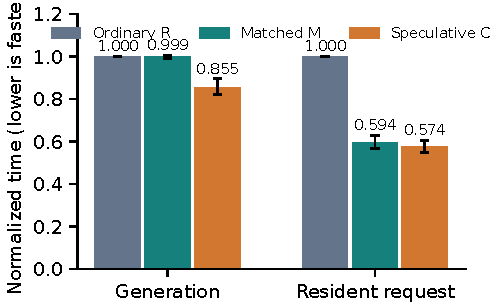
\includegraphics[width=0.62\linewidth]{figures/reference_cost.pdf}
\caption{RTX expansion costs normalized task-by-task to ordinary $R$, then geometrically averaged. Matched draft-free execution already reduces request cost substantially. Error bars invert the descriptive task-bootstrap intervals for $R/M$ and $R/C$. Bars are aggregate relative times, not additive cost components.}
\label{fig:reference}
\end{figure}

\begin{figure}[t]
\centering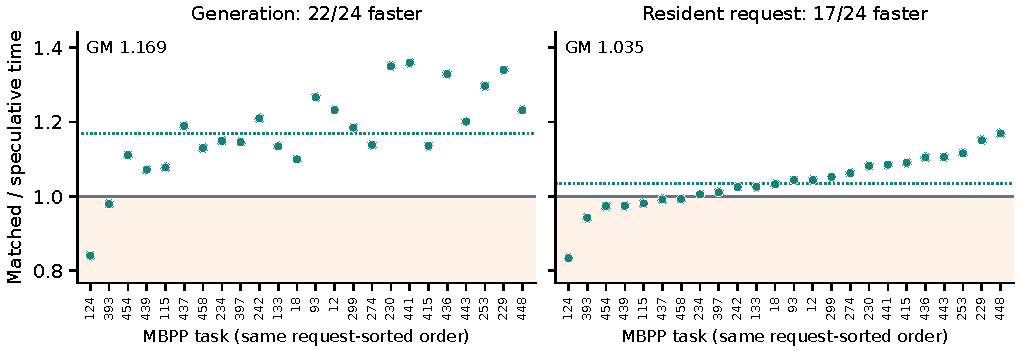
\includegraphics[width=0.96\textwidth]{figures/matched_task_effects.pdf}
\caption{RTX expansion: each point is the matched-target/candidate ratio of four-repetition absolute-time medians for one MBPP task. Both panels use the same order, sorted by request ratio. Generation improves on 22/24 tasks; resident-request time improves on 17/24. The line at one marks parity; the horizontal dotted line is the unweighted task geometric mean. Points are tasks, not independent repetitions.}
\label{fig:tasks}
\end{figure}

\subsection{Qualification and amortization boundaries}
Table~\ref{tab:boundary} summarizes the distinct outcomes. Passing the output gate does not imply passing the cost gate, and a failed output gate disqualifies a speed claim even if the recorded run is fast. The rows come from separate registered panels; they are not a pooled benchmark.
\begin{table}[t]
\centering\footnotesize\setlength{\tabcolsep}{3pt}
\caption{Observed qualification/cost combinations. Gen./req. speeds are against the named draft-free baseline; -- means no qualified speed claim.}
\label{tab:boundary}
\begin{tabular}{lccc}\toprule
Recipe & Qualified panel & Baseline & Gen./req.\\\midrule
RTX $k=3$, UB4 & 24 tasks & Matched & 1.169/1.035\\
RTX $k=7$, UB4 & 28 tasks & Matched & 0.997/0.950\\
RTX $k=7$, UB8 & Fails /229 & -- & --\\
B570 $k=2$ repair & 15 tasks & Ordinary & 0.283/0.201\\\bottomrule
\end{tabular}\end{table}
\subsection{Changing geometry can break the repair}
The expansion into draft length and microbatch capacity keeps failed cases. At paired $(k,\mathrm{UB})=(1,2)$ and $(3,4)$, the tested width/length panel qualifies. MBPP/229 fails at $(5,6)$ and $(7,8)$ under all measured cap contexts and repetitions, even though its wide ordinary and matched paths pass. The old HumanEval/18 probe also supplies an outside-panel failure at wider target-only capacity. Increasing the output cap does not certify every trajectory to that length: some responses finish much earlier, with observed maximum length 261 rather than a full 512-token stress trajectory.

A separate experiment holds UB4 fixed and tests $k=3,5,7$. All 28 exposed qualification tasks pass in two repetitions. The widest $k=7$ recipe is selected by qualification only, then measured in independent capture-off cost sessions. Against $k=3$, it obtains 0.82944$\times$ generation and 0.88987$\times$ request speed: qualified outputs, slower execution. Against matched target-only, $k=7$ reaches 0.99740$\times$ generation and 0.95035$\times$ request speed; the $k=3$ anchor reaches 1.20250$\times$ and 1.06797$\times$. Larger $k$ is neither a monotone correctness repair nor a monotone performance improvement in these contracts.

Diagnostic sessions, including warmup, record target caller calls falling from 305 to 199 while observed micrographs rise from 305 to 397. Separate formal work records show drafted tokens increasing from 3528 to 5392 and accepted tokens from 2772 to 3192. These are different sessions and must not be divided into one fabricated per-call measure. Micrograph observations are not CUDA kernel launches. The counts reveal why caller reduction is an inadequate performance proxy; they do not uniquely prove which component caused the slowdown. This limitation is consistent with prior work on verification cost~\cite{illusion}, while the fixed-capacity, reference-qualified counterexample adds a concrete numerical-contract boundary.

The resident serial-request study verifies reset behavior and positive finite costs on its own panel, approximately 1.181$\times$ generation and 1.039$\times$ request against its matched comparator. It is not a throughput or concurrency benchmark and is not pooled with the expansion.

\subsection{B570: repair without deployment gain}
The B570 frontend combines ordinary-reference prompt construction, in-place prefill-to-continuation phase binding from UB128 to UB1, and the existing $k=2$, draft-UB1 speculative loop. It qualifies 12 development requests, 112 requests over 56 exposed tasks, and all 30 candidate requests over 15 inputs unused in the accessible project. Qualification is the cap-128 endpoint contract from Section~\ref{sec:contracts}. The 30 candidate responses include extra raw suffix differences; endpoint equality cannot be rewritten as raw-array equality.

The formal E matrix is 119/120 complete because one old-N1 request lacks a payload. Ordinary $R$, matched target-only, and the candidate each have all 30 paid observations, so their 15 task-median pairs remain complete. Candidate speed is 0.28259$\times$ generation and 0.20129$\times$ request against ordinary $R$, slower in every paired round. Against matched target-only it is 0.28576$\times$ and 0.20570$\times$. Matched target-only itself is near the ordinary reference: 0.98889$\times$ and 0.97854$\times$. Thus the entire candidate regression cannot be attributed to a target consistency constraint alone.

Against 14 complete old-N1 task pairs, the candidate improves generation/request by 3.99309$\times$/2.63394$\times$, with a single request-round reversal at MBPP/245. This old-implementation improvement does not establish a deployable gain. Draft, accepted, caller and extra-suffix work are recorded, but no independent component profile identifies a unique remaining bottleneck. The measured recipe is a qualified cost failure; further optimization would require a different performance hypothesis.

\subsection{Global serialization as an earlier qualified cost failure}
An earlier RTX timing arm uses the same 19 exposed tasks as its prediction arm but 171 fresh observations: target-only UB1, batched speculation, and globally serialized speculation, each with three repetitions. Its direct-ID gate blocks batching at 51/57 arrays. Serialization qualifies at 57/57, yet its paired task-median speed is 0.677 times target-only, with descriptive interval [0.662,0.692] and zero of 19 prompts faster.

The global microbatch option also affects drafting. Its timer covers synchronized post-prefill work through slot release, including recorded sampler/state operations and logging. This is a different intervention and interval from the later attention-layout graph and server generation field. It cannot be combined with later results into a causal optimization trend. Its contribution is a separate qualified failure: global serialization preserved the tested reference but did not supply a useful latency operating point.

\subsection{Historical opportunities on M4 and 358H}
Historical M4 data supply a positive cost case. A prospective 60-task panel, 30 HumanEval plus 30 SpecBench~\cite{specbench} inputs, has three conditions and three repetitions: 540 requests. Fixed Always speculation and Guard each qualify 180/180 responses under that study's contract. Their post-prefill speedups against target-only are 1.34689$\times$ and 1.31139$\times$. Guard is 2.71\% slower than Always in geometric task latency. This guard has no measured advantage on the prospective panel.

A whole-request offline oracle choosing between target-only and Always by each observed task's medians improves on Always by only about 0.0692\% in geometric mean. It is a panel-specific choice oracle, not an upper bound for intra-request policies or other implementations. On Core Ultra 358H, CPU and NPU drafting reproduce the reference on their 90-request panels but yield 0.73392$\times$ and 0.35166$\times$ speed. Conditional removal of measured overhead leaves the available ceilings below parity. Full-prefix NPU replay and the historical target path are properties of that implementation, not impossibility results for heterogeneous decoding.


\subsection{Existing workload partitions reveal different operating points}
The fixed-UB width export separates 24 MBPP inputs and four HumanEval probes. Table~\ref{tab:strata} preserves these groups. At $k=7$, matched-target generation speed is 0.953 times on MBPP and 1.308 times on HumanEval; resident-request speed is 0.919 and 1.164 times. The pooled result is near generation parity and below request parity. Increasing width from $k=3$ remains slower in pooled costs, while the four-task HumanEval request result is approximately unchanged.

M4's separate prospective partition also has different gains: fixed speculation gives 1.570 times on HumanEval and 1.155 times on Spec-Bench. The guard reaches 1.555 and 1.106 times. The partitions illustrate why a global speed or accepted-token fraction does not specify which workload benefits. These are descriptive saved-data analyses, not a new adaptive method, validated routing rule, or CUDA/Metal comparison.
\begin{table}[t]\centering\footnotesize\setlength{\tabcolsep}{4pt}
\caption{Saved workload partitions. Speed is named baseline/candidate. RTX uses generation and resident-request timers; M4 uses its post-prefill timer. Rows are not cross-platform comparisons or independent validation panels.}
\label{tab:strata}
\begin{tabular}{llrlcc}\toprule
Study & Partition & Tasks & Comparison & Gen./post-prefill & Request\\\midrule
RTX width & MBPP & 24 & Anchor / wide & 0.806 & 0.873\\
RTX width & MBPP & 24 & Matched / wide & 0.953 & 0.919\\
RTX width & HumanEval & 4 & Anchor / wide & 0.985 & 1.000\\
RTX width & HumanEval & 4 & Matched / wide & 1.308 & 1.164\\
M4 & HumanEval & 30 & Target / fixed & 1.570 & --\\
M4 & HumanEval & 30 & Target / guard & 1.555 & --\\
M4 & Spec-Bench & 30 & Target / fixed & 1.155 & --\\
M4 & Spec-Bench & 30 & Target / guard & 1.106 & --\\
\bottomrule\end{tabular}\end{table}


\subsection{A target-work floor limits draft-only optimization}
The 358H measurements permit a conditional bound because complete target work was measured separately. For paired baseline cost $B_{ij}$ and target work $T_{ij}$, fixing progress and deleting all other nonnegative work implies
\begin{equation}
\operatorname{GM}_i\operatorname{median}_j S'_{ij}
\leq\operatorname{GM}_i\operatorname{median}_j(B_{ij}/T_{ij}).
\end{equation}
Prompt-estimator ceilings are 0.8372 times for CPU drafting and 0.8448 times for NPU drafting. Pooled-total ceilings differ: 0.8275 and 0.8352 times. Neither reaches parity. Even with other costs deleted, a uniform target-work reduction must reach at least 16.28\% or 15.52\% to make the prompt ceiling reach one. These are optimistic necessary budgets, not achieved improvements. Changed progress, target execution, or state interfaces require new qualification and measurement.

\section{System Design Implications}
\label{sec:discussion}
\subsection{Choose the control boundary before the repair}
The natural crosses show why token-prefix equality can hide a numerical dependency. A fixed current call does not erase previous numerical state; a fixed donor does not erase current-path sensitivity. The design decision is where a constraint must act: prefill, continuation, verification, reconciliation, or a combination. The measurements identify local candidates, not universal operators.

The early RTX intervention demonstrates the consequence of choosing too narrow a phase from an aggregate result. One task repairs and another regresses, even while prediction is exact. The later target-prefill/continuation family obtains a qualified operating point within its frozen graph. A repair argument needs both local diagnosis and native output qualification.

\subsection{Simpler paths define the value of added machinery}
The target-only bridge and matched comparator serve distinct related purposes. The bridge asks whether a complex reproducer supplies behavior unavailable from an ordinary path. The comparator asks whether speculation adds speed after changing the target path. Prediction accuracy and ordinary-reference speed alone cannot answer these questions.

RTX ordinary-reference resident-request speed is 1.742$\times$, while matched draft-free execution already gives 1.683$\times$. Speculation's increment is 1.035$\times$, with seven regressing tasks. It is a positive aggregate operating point with limited, uneven incremental request benefit. Its larger generation benefit covers a different interval.

\subsection{Qualification does not define a performance objective}
B570 endpoint repair succeeds as output recovery and fails as latency optimization against both draft-free baselines. Wider RTX drafting remains qualified at fixed capacity but lowers speed. On M4 a guard adds no measured advantage over fixed speculation; on 358H removing draft-side work alone cannot overcome the measured target-work floor.

These cases constrain different directions. They do not support a blanket instruction to serialize, enlarge drafts, add a controller, or offload drafting. Acceptance fraction, target-call count, and isolated draft throughput describe execution; none substitutes for paid request costs under a qualified output contract.

\subsection{What transfers and what remains specific}
The reusable contribution is the linked evaluation procedure: state/current-path controls, phase-scoped repair qualification, simpler output baselines, and ordinary/matched comparisons. Numerical recipes remain backend- and configuration-specific. CUDA and Vulkan do not share an unchanged proven repair, and M4/358H are not late-mechanism replications.

Workload partitions describe heterogeneity. Small or exposed subsets cannot validate a general selector. Cross-family experiments or shared-contract comparisons could extend the claim; more repetitions on an exposed panel would not establish that extension.


\section{Threats to Validity and Reproducibility}
Late mechanism and repair evidence predominantly uses Qwen3, greedy sampling, one slot, and recorded non-flash paths. Context, quantization, runtime, and driver belong to each configuration. Stochastic sampling, long-context generality, concurrent throughput, energy, and direct nearest-method comparisons are not established.

Selected-boundary probes target known sensitivity. They support local effects with shams, not prevalence across arbitrary requests. Selected tensor equality and complete-output equality do not prove universal state equivalence. Minimality concerns the registered switch family. B570 recipes change microbatch and output reservation jointly, preventing isolated operator attribution.

The expansion freezes inputs before references, but project exposure accounting cannot certify training-data independence. Repair selection uses exposed probes; width selection and width costs reuse tasks. Endpoints, task identities, and missingness remain campaign-specific. No pooled platform success rate or common latency trend is justified.

Laptop sessions can differ thermally and in scheduling. Balanced orders and medians expose variation but do not eliminate resident-session confounding. The second matched-request repetition reverses direction. Task intervals are not independent multi-day replication or population confidence intervals. Ordinary $R$ is paid and qualified but not shown globally fastest.

The source package separates frozen exports from new manuscript analysis. Its verifier checks saved arithmetic and hashes without model execution. Private raw authentication remains inherited from original hosts. Missing payloads, opaque sampler state, incomplete live target-only internals, and unavailable component durations remain explicit. Full replay requires omitted archives, weights, and runtimes.

\section{Conclusion}
Reference-preserving speculative execution requires both a qualified numerical trajectory and a useful paid operating point. Prediction closure and the target-only bridge show why reproducible intervention output alone does not establish repair utility. Natural-state/current-path crosses identify local dependencies hidden by equal prefixes. A finite RTX target-layout constraint supplies a qualified positive case, while ordinary and matched comparators reveal that most of its ordinary-reference request improvement is available without speculation.

Wider drafting, B570 endpoint repair, M4 adaptation, and 358H draft optimization expose distinct cost boundaries. Together, the cases support diagnosing the execution boundary, qualifying native output, and measuring deployment and incremental costs. Cross-family repair and broad deployment transfer remain open.

\section*{Data availability}
The author source package contains source-bound derived exports, historical extracts, and CPU verification scripts. It omits model weights, native runtimes, and some private raw archives. It supports arithmetic reproduction rather than independent hardware replay. The authors must finalize a persistent access location and additional raw-material availability before submission.

\section*{Declaration of generative AI and AI-assisted technologies}
OpenAI ChatGPT/Codex assisted with manuscript organization, drafting, and reproducible analysis code. Figures are retained from source-data analytical scripts; no generative image synthesis was used. This author-review draft requires final author verification, editing, and approval before submission; it does not represent completed author approval.


\label{maintextend}
\begingroup\small
\bibliographystyle{elsarticle-num}
\bibliography{references}
\endgroup
\end{document}

